\chapter{UI Overview}
\label{sec:ui_overview}

In this section, the main GUI components are described, to give an overview and introduce the different workflow options.

\subfile{ui_main_window}

\section{Main Menu}

\subsection{File Menu}
\label{sec:ui_overview_file_menu}

Databases can be created, opened and closed using the File menu.

\begin{figure}[H]
  \center
    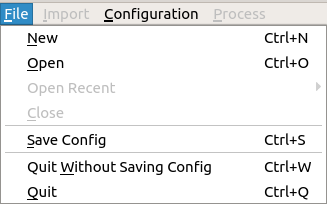
\includegraphics[width=6cm,frame]{figures/ui_file_menu.png}
  \caption{File Menu}
\end{figure}

\begin{itemize}
 \item New: Create new database file
 \item Open: Open existing database file
 \item Open Recent: Open recent existing database file
 \item Close: Close current database
 \item Save Config: Save current configuration
 \item Quit Without Saving Config: Quit application without saving configuration
 \item Quit: Quit application with saving configuration
\end{itemize}
\  \\

After a database was opened, the 'Import' menu becomes available, and the main window looks as follows:

\begin{figure}[H]
  \hspace*{-2.5cm}
    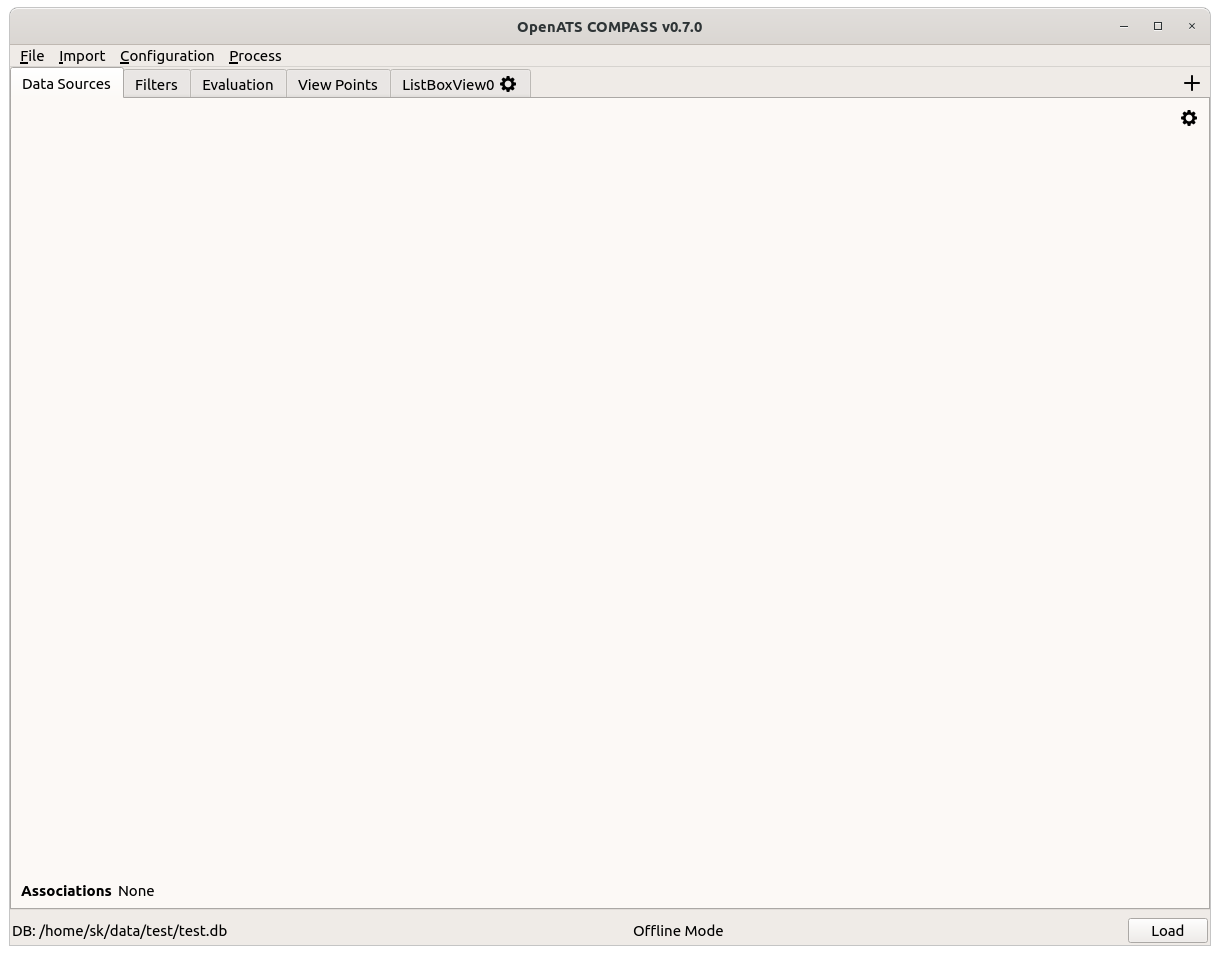
\includegraphics[width=19cm]{figures/main_window_opened.png}
  \caption{Main Window After Opening a Database}
\end{figure}

\subsection{Import Menu}
\label{sec:ui_overview_import_menu}

Data can be imported into the database using the Import menu. This menu is only accessable if a database was opened.

\begin{figure}[H]
  \center
    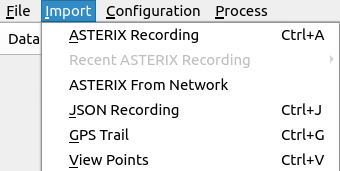
\includegraphics[width=6cm,frame]{figures/ui_import_menu.png}
  \caption{File Menu}
\end{figure}

\begin{itemize}
 \item ASTERIX Recording: Import ASTERIX recording file
 \begin{itemize}
 \item see \nameref{sec:ui_import_asterix}
 \end{itemize}
 \item Recent ASTERIX Recording: Import recent ASTERIX recording file
  \begin{itemize}
 \item see \nameref{sec:ui_import_asterix}
 \end{itemize}
 \item ASTERIX From Network: Import ASTERIX from network interfaces in Live mode
  \begin{itemize}
 \item see \nameref{sec:ui_import_asterix_network}
 \end{itemize}
 \item GPS Trail: Import (D)GPS trail from NMEA file
  \begin{itemize}
 \item see \nameref{sec:ui_import_gps}
 \end{itemize}
 \item View Points: Import View Points definition file
  \begin{itemize}
 \item see \nameref{sec:ui_import_viewpoints}
 \end{itemize}
\end{itemize}
\  \\

\subsection{Configuration Menu}
\label{sec:ui_overview_config_menu}

Data sources and sectors can be configurated using the Configuration menu. Also, the current Meta variables can be inspected.

\begin{figure}[H]
  \center
    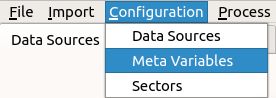
\includegraphics[width=5cm,frame]{figures/ui_configuration_menu.png}
  \caption{Configuration Menu}
\end{figure}

\begin{itemize}
 \item Data Sources: Configure data sources
  \begin{itemize}
 \item see \nameref{sec:ui_configure_data_sources}
 \end{itemize}
 \item Meta Variables: Display current Meta variables
  \begin{itemize}
 \item see \nameref{sec:configure_meta_vars}
 \end{itemize}
 \item Sectors: Configure sectors in the database
  \begin{itemize}
 \item see \nameref{sec:ui_configure_sectors}
 \end{itemize}
\end{itemize}
\  \\

\subsection{Process Menu}
\label{sec:ui_overview_process_menu}

Post-processing tasks can be performed using the Process menu. This menu is only accessable if a database was opened.

\begin{figure}[H]
  \center
    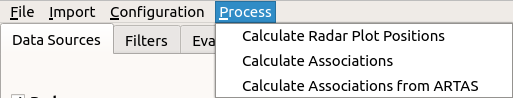
\includegraphics[width=10cm,frame]{figures/ui_process_menu.png}
  \caption{Process Menu}
\end{figure}

\begin{itemize}
 \item Calculate Radar Plot Positions: (Re-)Calculate Radar plot position information
   \begin{itemize}
 \item see \nameref{sec:ui_proc_radar_plot_pos}
 \end{itemize}
 \item Calculate Associations: Find unique targets and associate target reports
   \begin{itemize}
 \item see \nameref{sec:ui_associate_tr}
 \end{itemize}
 \item Calculate Associations from ARTAS: Find targets based on ARTAS tracks and associate target reports based on ARTAS TRI information
   \begin{itemize}
 \item see \nameref{sec:ui_associate_tr_artas}
 \end{itemize}
\end{itemize}
\  \\

\subfile{ui_import_data}
\subfile{ui_configuration}
\subfile{ui_postprocess}
\subfile{ui_data_sources}
\subfile{ui_filters}
%\subfile{ui_use_cases}

% \subfile{task_manage_schema}
% \subfile{task_manage_dbo}

% \subfile{task_import_json}

\subsection{Views}
The 'Add View' button \includegraphics[width=0.5cm,frame]{../../data/icons/crosshair_fat.png} on the top right in each window allows adding views to the current window or in a new window. \\

Each View is contained in a tab within a parent window.  At startup, per default only the main window exists, which also holds
a ListBox view. If the main window is closed, the COMPASS client shuts down. New Views can be added using the 'Add View' button, which opens a pull-down menu. Each View can either be added to the main window ('Add Here') or into a new window ('Add in New Window'. When added, a new tab exists in the containing window. \\

New Views can be added either to currently existing windows as new tabs, or to a newly opened window. A window can be closed either by the close button in the window decoration, which discards all contained Views within the window.  \\

To close a single View, one can use the \includegraphics[width=0.5cm,frame]{../../data/icons/edit.png} button in the tab header, which frees up all its allocated resources. \\

Each View adds its required variables to the loading list for the database. During a loading process, the loading status  of a View is shown in the management tab.\\

Currently, the following Views exist:
\begin{itemize}
 \item \nameref{sec:histo_view}
 \item \nameref{sec:listbox_view}
 \item \nameref{sec:osg_view}
 \item \nameref{sec:scatter_view}
\end{itemize}

